\documentclass{article}

% Language setting
% Replace `english' with e.g. `spanish' to change the document language
\usepackage[english]{babel}

% Set page size and margins
% Replace `letterpaper' with `a4paper' for UK/EU standard size
\usepackage[letterpaper,top=2cm,bottom=2cm,left=3cm,right=3cm,marginparwidth=1.75cm]{geometry}

% Useful packages
\usepackage{amsmath}
\usepackage{graphicx}
\usepackage[colorlinks=true, allcolors=blue]{hyperref}
\usepackage{caption}
\usepackage{subcaption}
\title{Plenoxels and extension to point clouds}
\author{Nissim Maruani}

\begin{document}
\maketitle

\begin{abstract}
\cite{plenoxels}
\cite{nerf}
\cite{spacecarving}

\cite{directvoxgo}
\cite{instant}
\end{abstract}

\section{Introduction}

The most straightforward way to capture 3D objects from the real world requires special sensors such as the Kinect or more expensive scanning devices. Another approach only relies on RGB images: by intersecting the information taken at several known viewpoints, one is able to render novel views of a scene. A year ago, a method known as \textit{NeRF} (for Neural Radiance Field \cite{nerf}) tackled this challenge by using a deep neural network to simultaneously shapes and shadings. More recently, a new approach \cite{plenoxels} showed that directly optimizing a voxel grid (known as \textit{Plenoxels}) allowed better results with faster computations. This project is focused on this paper. We re-implemented parts of it and showed that its method can be extended to generate point clouds from photographs.  

\section{Our implementation}

\subsection{Given code}


The given code associated to the plenoxels paper requires the compilation of a custom CUDA extension which parallelizes across rays, opacities and spherical harmonics coefficients. Unfortunately, it requires a CuDNN developer account and quite a bit of C++ experience (another alternative relies on JAX, but is much slower to train). In order to avoid losing time on hazardous compilations, we decided to code everything \textbf{from scratch}, except for the following elements:
\begin{itemize}
\item The utilities functions \textit{get\_data} and \textit{get\_rays\_np} (30 lines of code) from the original plenoxels repository \footnote{https://github.com/sxyu/svox2}

\item The Python file \textit{ply.py}, given in the TP of this course.  

\end{itemize}

\subsection{Our implementation}


Since our implementation is "homemade", it doesn't contain every extension described in the paper. It is slower (because it doesn't use a custom CUDA kernel), but it also much easier to run (a simple TODOx128x128 grid can be trained in TODO time). Our code is organized in the following manner:


\begin{itemize}
\item The file \textit{VoxelGrid.py} contains the different voxel grids (RGB colors, spherical harmonics and tri-linear interpolation) 
\item The files \textit{main.py} and \textit{main\_spherical.py} are used to optimize our grids
\item The different jupyter notebooks allow for a more interactive training and computation of PSNR
\item Some useful functions (including \textit{get\_data} and \textit{get\_rays\_np}) are located inside \textit{utilities.py}.
\end{itemize}

The Plenoxel paper introduces remarkable concepts and the given implementation is no less great: reproducing the results was a challenge, and improving the given method (in terms of speed or quality of results) was impossible in the scope of this project. However, we found a way to extend this approach by integrating a point cloud export to the code, which links this project to the NPM3D course.   

\subsection{Datasets}

TODO

\section{Related works}



\subsection{Classical methods}

Before the rise of neural networks, some methods already existed to render novel views from images: one of them is called \textit{Space Carving} \cite{spacecarving}. This method successfully captures the 3D shape and texture of the photographed scenes, but is unable to render the shading and capture the specular properties of the objects. However, we noticed the rigor of the authors who provide theoretical guarantees, absent from \textit{NeRF} or \textit{Plenoxels}.

\subsection{NeRF rendering}

The \textit{NeRF} \cite{nerf} approach consists of training a fully-connected network which takes a 5D input $(x,y,z,\theta,\phi)$ composed of a 3D position and a viewing direction, and outputs a 4D tensor $(r, g, b, \sigma)$ composed of an RGB color and an opacity $\sigma$. For each pixel of the rendered image, $N$ points are sampled along a camera ray and their colors and intensities are integrated to obtain a final $RGB$ value. This method achieved state-of-the-art when it was published, as it allowed to reproduce shading and specular effects efficiently. The training time, however, was quite slow (12 hours for a single scene).

\subsection{Concurrent papers and posterior approach}

\textit{DirectVoxGo} \cite{directvoxgo} is similar to Plenoxels: the main differences are that it uses a neural network (and not a custom CUDA implementation). It produces NeRF-comparable results in less than 15 minutes. More recently, a method using multiresolution Hash encoding \cite{instant} was able to reproduce the same results in less than 1 second!

\section{The method}

In this section, we'll describe the method of the original paper \cite{plenoxels}, and list the different between their implementation and ours (see Figure \ref{fig:plenoxel}).



\begin{figure}[!h]
\centering
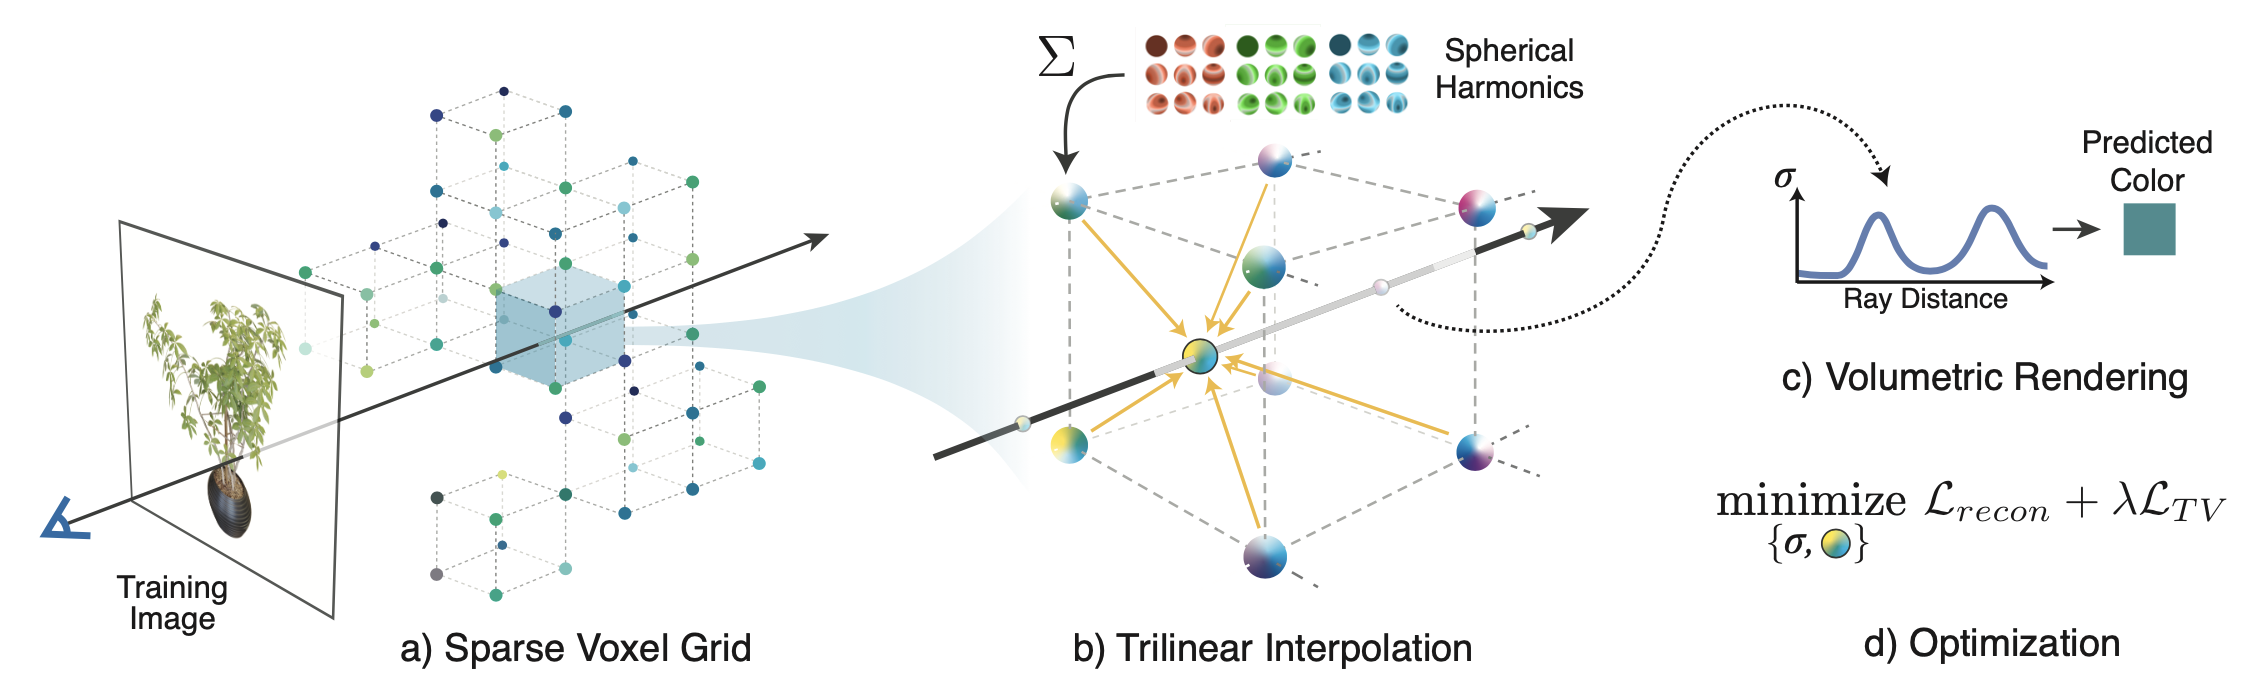
\includegraphics[width=1.\textwidth]{figs/plen_pipeline.png}
\caption{\label{fig:plenoxel} [image source: \cite{plenoxels}] We implemented a simpler version of the the full plenoxel pipeline. First we extract camera rays from training images and sample them on a dense (not sparse) voxel grid (a). Then we compute the spherical harmonics (or simply the RGB colors if the desired output is a pointcloud) for each sample through nearest neighbor interpolation (and not trilinear interpolation) (b). Finally we sum the resulting colors and opacities to obtain a single pixel value (c), and optimize it with a total variation regularizer (d).}
\end{figure}



\subsection{The voxel grid}

The clever idea of Plenoxels is to optimize a voxel grid directly. Each voxel stores an opacity $\sigma \in \mathbf{R}^+$ along with spherical harmonics coefficients in $[0,1]$ (in the original paper they use 9, but we used 4 to optimize computations). These spherical harmonics allow each voxel to have a different color depending on the viewing direction, which renders specular effects and reflections.

The original paper uses a sparse voxel grid optimized with the custom CUDA implementation. Ours is a dense voxel grid which which justifies the lower definition (128x128x128 vs 512x512x512) and the longer computation time of our implementation.

\subsection{Color estimation from camera rays}

Once this grid is initialized at random, we optimize its voxels based on images taken from known viewpoints. Each pixel $p_x$ of the training images corresponds to a certain camera ray $r(p_x) \in (\mathbf{R}^3, \mathbf{R}^3)$ composed of an origin and a direction. We sample this ray with $N=200$ points, compute the points colors and opacities via nearest neighbour interpolation (we implemented trilinear interpolation like in the paper but it was 8 times slower) and sum the sampled points to obtain the estimated RGB color $\hat{c}(r(p_x))$:
\[\hat{c}(r(p_x)) = \sum_{0\leq i<N} T_i (1 - \exp(-\sigma_i \delta_i)) c_i\] 

Where $ T_i = \exp(- \sum_{0\leq j<i} \sigma_j \delta_j)$ represents how much light is transmitted to sample $i$ and $\delta_i$ represents the distance between samples.


\subsection{Optimization}
Then it suffices to use back-propagate the mean squared error loss with total variation regularization: $L = \sum_{p_x} \|p_x -\hat{c}(r(p_x)) \|^2 + \lambda_{TV}  L_{TV}$. At each training step, we sample 5000 random rays and compute the total variation over the whole grid. We used an SGD optimizer to do the gradient descent with a learning rate of 1000, and $\lambda_{TV} = 10^{-4}$. 

\section{Using plenoxels to generate point clouds}

\subsection{Point cloud generation}

\subsection{CloudCompare pipeline}


\begin{figure}[!h]
 \centering
\begin{subfigure}{.45\textwidth}
  \centering
  % include first image
  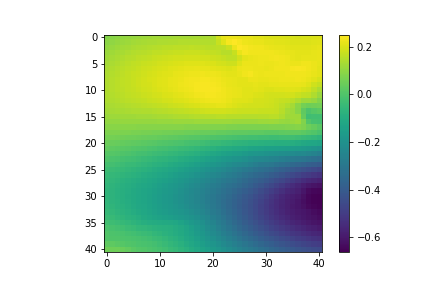
\includegraphics[width=\linewidth]{figs/corr1_.png}  
  \caption{Corrélations pour la ville 1}
         \label{fig:raw}
\end{subfigure}
\begin{subfigure}{.45\textwidth}
  \centering
  % include second image
  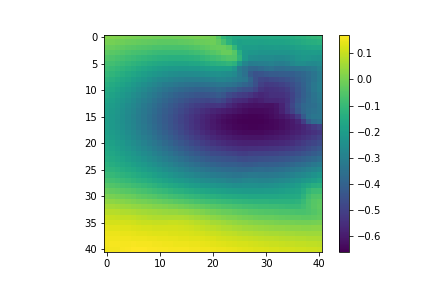
\includegraphics[width=\linewidth]{figs/corr2_.png}
  \caption{Corrélations pour la ville 2}
         \label{fig:rotated}
     \end{subfigure}
     \caption{Corrélations entre la surcote et la pression}
    \label{fig:corr}
\end{figure}




%\begin{figure}
%\centering
%\includegraphics[width=0.3\textwidth]{frog.jpg}
%\caption{\label{fig:frog}This frog was uploaded via the file-tree menu.}
%\end{figure}


%\begin{table}
%\centering
%\begin{tabular}{l|r}
%Item & Quantity \\\hline
%Widgets & 42 \\
%Gadgets & 13
%\end{tabular}
%\caption{\label{tab:widgets}An example table.}
%\end{table}

%\url{https://www.overleaf.com/contact}.
%\href{https://www.overleaf.com/user/subscription/plans}{upgraded account}
\bibliographystyle{alpha}
\bibliography{sample}
\end{document}